\documentclass{article}
\usepackage{graphicx} % Required for inserting images
\usepackage{url}
\usepackage{hyperref}
\usepackage{amsmath}
\usepackage{csquotes}
\usepackage[margin=1in]{geometry}

\title{Quantifying Uncertainty in College Basketball}
\author{Seth Peacock, Jake Browning, Rohan Mawalkar}
\date{November 17 2024}

\begin{document}

\maketitle

\newpage

\section{Letter to the Editor}
% In addition to this report, write a one-page letter to the newspaper chief editor, explaining the main results of the report and suggesting findings that can be communicated with the basketball fans reading the newspaper.

People love sports because they are a showcase of hard work and talent. People also love sports because they are unpredictable. How do we quantify the effect of one versus the other in a basketball game? On the one hand, we often see this framed as a strict dichotomy between luck and skill: sports outcomes depend in some part on one and in some part on the other. However, careful examination reveals that it is rather unclear where to draw the line between luck and skill. For example, if a team happens to study exactly the right film the night before a big game and is able to perfectly foil the other team's plans, is that luck or is it skill? On the one hand, it certaintly takes skill to study your opponent and use this information to your advantage. On the other hand, they could have easily picked the wrong film to study! Instead, it is better to approach this problem using a dichotomy between certainty and uncertainty. Certainty is how sure we can be about the outcome of a game using past data (ranking, players' stats, etc). But if you utilize all the data available to you, and there's still some chance of an upset, that means there's still some uncertainty in the outcome.

Year after year, people fill out brackets to try to predict the March Madness tournament. Year after year, not a single person is able to correctly guess the whole thing~(\cite{cbsnewsAnyoneEver}). This is a clear indication that the tournament is just too uncertain to expect to be able to predict. We're not claiming anything deeply metaphysical here. It could be true that if you knew the precise location of all the relevant atoms in all the stadiums and in all the players and in everything they interact with then you could predict the outcome of the NCAA tournament perfectly. The question we are interested in is different: \textit{given the data we have}, what is the minimum amount of uncertainty that still exists in a basketball game? That is, what is the minimum chance of an upset, no matter how different in observed skill two teams are?

The first step in our approach is to assign ratings to each team. We do this via a modified version of the classic Elo rating system in chess. Each team starts at the same Elo rating. We then walk through the regular season game by game, and after each game we update the Elo rating of each team based on three factors: whether the team won or lost, by how many points, and the Elo rating (how ``good'') the other team was. If you win, your rating goes up, and if you lose it goes down. If you win/lose in a blowout, it would go up/down a lot. If you beat a team that's much better than you, you go up by a lot, while if you beat a team that's much worse than you (or lose to a team much better than you), you don't change much. 

After stepping through all games in the season, we hope that our ratings are reasonably accurate. The beauty of the Elo ratings is that they inherently provide the expected probability of an upset given a skill level difference. Therefore to verify our end of season ratings, we can look at all of the games with a given skill level difference, and compare the predicted probability of an upset to the observed percentage of those games which had an upset. If these are close, this is a good indication that our ratings are accurate.

Now that we have our ratings, there are two things we can do with them. First, we can go ahead and simulate the tournament. For each game in the bracket, we calculate the probability of an upset based on the difference in their Elo ratings. We then ``roll a die'' to find out if there was an upset, based on the previously calculated probabilty. For example, say a 6 seed is playing a 11 seed in the first round. Based on the Elo rating differential (NOT based on the seeds, which any basketball fan will tell you are poor estimations of actual skill), we calculate that the probability of an upset is 1/6. We then roll a die --- if it lands on 6, we say there is an upset and the 11 seed wins. If it lands on anything else, we say the 6 seed wins.

We are not claiming that running this simulation will predict the outcome of the tournament. After all, we're still picking the winners by rolling a die (even if it's a weighted one)! The best we can do is come up with a model that can at least tell you what tournaments like this one could look like, which perhaps isn't of much interest to your readers. However, our original question was about the minimum amount of uncertainty in a basketball game. This we can now begin to answer. First, we find the biggest Elo score differential that we found to exist between two teams. Next, we look at all of the past games between two teams that were this maximum distance apart in skill, and estimate the probability of an upset in this category. Ideally, \textit{this percentage is then our desired minimum uncertainty}. For us, we found this number to be between 0 and 0.0538 with approximately 95\% certainty. 

There's just one problem: we were looking for the minimum amount of uncertainty \textit{when all of the available data was used.} Whatever constitues \enquote{all of the available data} is going to be a massive store created over the past decades which we have neither the time, resources, or access to process. We only used scores for the 2024 regular season games. Ideally, we would also incorporate scores for past seasons (especially past tournament games), assign Elo rankings to individual players, consider injuries, and so on. All of this is certainly doable, but is beyond the scope of our project. The more data we incorporate, the less this expected minimum uncertainty should be. However, unless we get to the point where we're tracking the precies positions of all of the atoms, this minimum upset probability will always be nonzero. Since we live in a world where any mention of the bizzarities of quantum mechanics scintillates the masses, we'll make the comparison before someone else does: perhaps it would be apt (if not scientifically founded) to think of the ideal minimum upset probability as the manifestation of a \enquote{basketball uncertainty principle.}

\newpage

\section{Overview}
% Describe the problem, your model, results and how your model performed.

The primary question we are interested in is: \textit{given the data we have}, what is the minimum amount of uncertainty that still exists in a basketball game? That is, what is the minimum chance of an upset, no matter how different in observed skill two teams are?

The first step in our approach is to derive this ``observed skill'' by assigning ratings to each team. We do this via a modified version of the classic Elo rating system in chess. Each team starts at the same Elo rating. We then walk through the regular season game by game, and after each game we update the Elo rating of each team based on three factors: whether the team won or lost, by how many points, and the difference in Elo ratings. For example, a team's rating will go up more if they beat a team that's better than them, and go up even more if they beat that team by a large margin. We experimented with several ways of incorporating this score differential.

After stepping through all games in the season, we want to verify the accuracy of our ratings. We first partitioned the games by score differential. The Elo rating system gives an expected probability of an upset for every possible score differential, so assign an expected upset probability for each partition by using the Elo expectation for the middle differential in that partition. For example, for the partition of (100, 125) we would use the Elo expected upset probability for a score differential of 112.5. We then looked at all of the actual games that fell into that partition, and calculate the percentage of them where an upset occurred (defined as the team with the lower Elo rating winning). This we take as an MLE estimate for the true probability of an upset for that score differential category~\cite{statproofbookMaximumLikelihood}. We then compare these observed and expected probabilities by plotting them on a 2D scatterplot and calculating the MSE from the $y=x$ diagonal. The closer these two values are, the closer they will be to the diagonal, which will be a good indication that our ratings are accurate. 

When defining our Elo updates, we had a parameter $K$ which was originally arbitrarily chosen. We can now repeat this entire process for multiple values of $K$ and pick the one that results in the lowest MSE.\@ We tried various values of $K$; the lowest MSE was obtained when $K\approx80$ and which yielded a minimized value of $MSE\approx0.0458$. (See \autoref{fig:MSE vs K}) This $K$ was larger than the canonical range, which is $K \in[10, 40]$~\cite{mediumRatingSystem}. Interestingly, for this value of $K$ the Elo estimate and the MLE estimate agreed for high score differentials, but for small score differentials the Elo estimate predicted a higher probability of an upset than the MLE estimate. (See \autoref{fig:Elo vs MLE}; note that dots with the higher Elo upset probability estimate necessarily correspond to the partitions with smaller score differentials by definition.)

We continue with this value of $K$ and the corresponding Elo ratings in hand, knowing that we have some validation for these ratings. There is one partition we are particularly interested in: the one for the largest score differentials. (In our case, we chose this to be all games with a score differential of 500 or more; see \autoref{fig:bootstrap dist}). We use bootstrapping to estimate an approximate 95\% confidence interval for the probability of an upset in this partition. That is, we sample with replacement from all of the games in the partition, giving us a sample mean. We do this over and over until we have a bootstrapped distribution for the sample mean. We then take the middle 95\% quantile of this distribution as our approximate 95\% confidence interval for the true probability of an upset in this category~\cite{uchicagoPercentileBootstrap}. We found this interval to be $[0, 0.05376]$. The fact that zero is included in the interval is not ideal, but perhaps could have been acheived by bootstrapping more samples (we only did 10,000).With the (significant) assumptions described in \autoref{bootstrapping}, this represents the ``baseline uncertainty'' of a basketball game: even in the case with the biggest observed skill difference --- the most certainty about the game --- this is the minimum probability of an upset. 
\newpage

\section{Introduction}
% ``Rephrase the problem
% Problems are open-ended and there are many ways to interpret and address them. Explain how you approached the problem."
In this paper, we explore the relationship between skill and luck in college basketball. Our goal here is twofold: first we develop a model which predicts the outcome of a basketball game, and second we use this model to somehow quantify the significance of luck/uncertainty in a basketball game. Since we want to incorporate the effect of uncertainty, our prediction model will contain a stochastic element which we will have to derive. To train our model, we will use data from the regular season games leading up to the 2024 March Madness Tournament, and then test our model's ability to predict the outcome of the tournament. Of course, we do not expect to be able to actually predict the outcome of the tournament. We won't go as far as to say that this is impossible; it could be true that if you knew the precise location of all the relevant atoms in all the stadiums and in all the players and in everything they interact with (etc.) then you could predict the outcome of the NCAA tournament perfectly. If this is true, then it may be accurate to say that there is no such thing as ``luck'' in basketball (depending on how you define luck). We will set this aside, as the question we are interested in is different: \textit{given the data we have}, what is the minimum amount of uncertainty that still exists in a basketball game? More concretely, what is the minimum chance of an upset, no matter how different in skill we observe two teams to be? We will use our model to estimate this minimum upset probability.

\section{Methods}
% ``Explain your model
% Clearly state and justify ALL assumptions your model uses
% Motivate your model. Why did you choose your approach?
% Clearly describe your model
% Clearly define all variables
% Include tables and figures to make it easier to understand
% Analyze your model
% What are the strengths and weaknesses of your model?
% How could you test your model? How stable are the results to noise? 
% If you had more time, how would you expand/improve your model''?

Our model will implement modified version of the classic Elo ranking in chess. Using win/loss and score data from the 2024 regular season, we assign each team a ranking. (From here on, when we say ``Elo ranking'' we will mean our modified ranking, and will be more specific if we mean the original.) Given a pair of teams, these rankings will be used to give us probabilities of an upset (that is, the probability that the team with the lower Elo rating wins). 


\subsection{Our ``Elo'' Ranking}
Traditionally, (see~\cite{mediumRatingSystem}), the Elo ranking system first calculates an expected score for the game as a function of the difference in the two teams' Elo ratings. Here, $E$ is the probability that the ``main'' team wins, while $E_{opp}$ is the probability that the opposing team wins:

\begin{equation}\label{eq:E}
E = \frac{1}{1+10^{(\gamma_{opp}-\gamma_n)/c}}
\end{equation}
\begin{equation}\label{eq:E_opp}
E_{opp} = \frac{1}{1+10^{(\gamma_n-\gamma_{opp})/c}}
\end{equation}

where $\gamma_n$ is the main team's pre-game Elo score (after game $n$), $\gamma_{opp}$ is the opposing team's pre-game Elo score, and $c, K > 0$ are constants. Note that $E + E_{opp} = 1$. The main team's Elo rating is updated after their $n+1^{\text{th}}$ game based on the following formula:

\begin{equation}
\gamma_{n+1} = \gamma_n + K(O - E)
\end{equation}


Where $O$ is 1 if the team wins and 0 if the team loses. Since E is a probability,  $E \in [0, 1]$. This means that a team winning or losing uniquely determines whether they gain or lose points on their Elo rating. This is essentially performing a stochastic gradient descent (taking a step after each game) for a logistic regression model, where the Elo ratings are the weights of the model~\cite{stmorseStatisticalLearning}.

However, this traditional Elo score update does not take into account the score differential of the outcome of the game, given its origin in chess, a scoreless game. Thus we propose a modified Elo system which uses the score outcomes to update a team's Elo score in following way: 


\begin{equation}
\label{multiplyUpdate}
\gamma_{n+1} = \gamma_n + K(O - E)\frac{S_{\text{win}}}{S_{\text{lose}}}
\end{equation}


where $S_{\text{win}}$, $S_{\text{lose}}$ are the scores of the winner/loser and the other variables are defined as above. These changes mean that a team's Elo rating will change by a larger amount when the score differential is larger, allowing for larger changes (positive or negative) in the case of a blowout. We will calculate $E$ in the same way as setting $c$ to the canonical 400 for simplicity, and choose $K$ based on considerations described in the next section near a canonical value  of $K\approx 32$~\cite{mediumRatingSystem}.

We considered several possibilities for incorporating the score differential. We could have defined the score differential as the absolute value of the difference of the scores. However, this would weight a 20--10 loss as the same as a 90--80 loss, which seems incommensurate with how basketball fans see the game. Thus, we would like to instead use the ratio $\frac{S_{\text{win}}}{S_{\text{lose}}}$. The question now becomes: how much do we want to allow this ratio to effect the score update? We also originally experimented with an exponential effect:

\begin{equation}
    \label{exponentialUpdate}
    \gamma_{n+1} = \gamma_n + K^{\frac{S_{\text{win}}}{S_{\text{lose}}}}(O - E)
\end{equation}

However, the exponential update caused certain teams to have a drastically different Elo ranking, which made our later analysis (such as partitioning games by score differential) difficult. See \autoref{rejectedideas} for more details.

\subsection{Elo Calculation Algorithm}
Our goal is to have an Elo ranking for every team that made it to the 2024 March Madness Tournament, using the results of the games in the regular season. However, many of these regular season games were not played against the teams that made it to the tournament. Thus, we also needed to assign Elo ratings to teams that did not play in the regular season. Note that there aren't many games for these non-tournament teams; we will discuss this issue below. 

We start all teams at the same Elo rating. This is typically a high positive value (to prevent giving a discouraging negative rating to low ranking chess players), but since the model solely uses the difference in Elo ratings, it doesn't matter what the initial value is. We chose to set it at 0 for simplicity. We then sort the games by date, and use \autoref{multiplyUpdate} to update the Elo ratings for every game. After all of the games have caused updates, we now have the Elo rating for every team that made it to the tournament (and some other teams as well).


\subsection{Verifying Elo Rankings}\label{verify}
We would like to verify the accuracy of our Elo system. To do this, we go back to the samples from the regular season games to compare our model's predictions of the probability of an upset to the actual observed probability of an upset, for a given difference in Elo rankings. 

First, we then partition the games based on these score differentials. For each partition, we then calculate $E_u(\Delta_{\text{Elo}})$ via \autoref{eq:E} using the middle $\Delta_{\text{Elo}}$ for that partition. Let $N_i$ be the number of games played in the regular season. To calculate $\hat{p}_u(\Delta_{\text{Elo}})$, we simply take the number of upsets (lower Elo rating team wins) divided by $N_i$. This is the maximum likelihood estimate (MLE) for the probability of an upset in the given partition~\cite{statproofbookMaximumLikelihood}.




To quantify the accuracy of our Elo system, we first plot the Elo predicted upset probability $E_u(\Delta_{\text{Elo}})$ against the observed probability MLE $\hat{p}_u(\Delta_{\text{Elo}})$ for each value of $\Delta_{\text{Elo}}$. We then plot the $y=x$ line and calculate the MSE of these points with respect to this diagonal line. That is, we calculate the straight line distance from each point in 2D space to the $y=x$ line~\cite{enwiki:1235411332}:

\[
D_i = \frac{|E_u(\Delta_{\text{Elo, i}}) - \hat{p}_u(\Delta_{\text{Elo, i}})|}{\sqrt{2}}
\]

and average the squares of these distances:

\[
MSE = \frac{1}{M}\sum_{i=1}^M {(D_i)}^2
\]

where $M$ is the number of partitions. We then repeat this process for a range of $K$ values, and choose the $K$ that minimizes the MSE.\@ (See INSERT REF TO PLOT.) Of course, this process increases the risk of overfitting to the regular season data. However, if we incorporate the tournament games, then we are not providing an unbiased assessment of our model's performance on the tournament data. See \autoref{nextSteps} for further discussion of overfitting. For a histogram of the distribution of score differentials in games for the value of $K$ we ultimately settled on, see \autoref{fig:K histogram}.

\begin{figure}[!htb]
    \begin{center}
      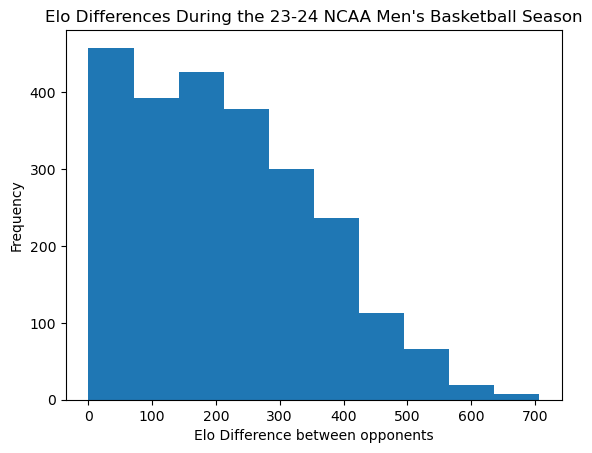
\includegraphics[width=0.5\textwidth]{K histogram.png}
    \end{center}
    \caption{Histogram of all the score differentials with $K=80$.}\label{fig:K histogram}
\end{figure}

\subsection{Bootstrapping the Baseline Uncertainty in Basketball}\label{bootstrapping}
As alluded to in the introduction, there is one partition we are particularly interested in: the one with the highest score differential. We will bootstrap many sample means to construct an approximate 95\% percentile bootstrap confidence interval (CI) for the probability of an upset in the highest score differential partition(see~\cite{uchicagoPercentileBootstrap},\cite{hesterberg_bootstrap_2015}). This will give an approximate 95\% CI for the ``baseline uncertainty'' of a basketball game in the March Madness tournament, provided we make the following assumptions:
\begin{enumerate}
    \item The Elo rating system is able to accurately capture all of the certainty that is currently able to be gleaned from pre-tournament data.
    \item The ELo rating system \textit{has} accurately captured all of the certainty that is currently able to be gleaned from pre-tournament data.
    \item This maximum Elo rating difference is close to the true maximum Elo rating difference that would happen in a tournament. 
    \item This sample of high differential games is representative of all high differential games.
    \item The sample distribution of the sample mean is symmetric (this allows us to say we can cut off both 2.5\% tails of the distribution for our confidence interval).
    \item The bootstrapped sample distribution of the sample mean is representative of the true distribution of the sample mean.
\end{enumerate}

If are comfortable with these assumptions, we would then have an estimate range for the minimum amount of uncertainty that exists a tournament game, regardless of skill differential. With more time, we would have liked to explore the validity of these assumptions in more detail. We discuss the most glaringly obviously unsatisfied one in the next section.


% 3. POSSIBLY Use the CI for p-hat to adjust Elo ratings and/or accept/reject a hypothesis about the actual p-hat.



\subsection{Weaknesses}
An obvious weakness of our model is our lack of data for the other teams in the league. Ideally, we would like to have accurate Elo ratings for these teams so that we can get accurate Elo updates for the tournament teams. We have tried to address this by changing the update formula for non-tournament teams, but ultimately we would prefer to just have more data for those teams. But this is just a small part of the problem; clearly, there is much much more pre-tournament data out there that could be useful, and assumption \#2 above is false. All we are using in our model is the win/loss margins of the regular season games. For this reason, we do not claim that our observed derived minimum amount of uncertainty is an accurate estimate of the true uncertainty when all currently available data is utilized. The more information used, the more opportunities there are to turn uncertainty into certainty. Our claim is that this is an estimate for the uncertainty \textit{given the data we used}. We discuss different types of data we could incorporate in \autoref{additionalData}. Another weakness is the previously mentioned risk of overfitting to the regular season data due to the selection of $K$. We explore possible solutions in \autoref{nextSteps}.

\subsection{Rejected Approaches}
We considered only using the games between tournament teams to caluclate the MLE of each partition upset probability. However, this would have seriously limited our already small dataset, so we decided against this. 

As previously mentioned, we also considered using an exponential Elo update. We had planned to use this in particular situations, depending on whether or not the teams involved were tournament teams. We considered four situations:

\begin{enumerate}
    \item The update for a tournament team after beating a non-tournament team. In this case we use \autoref{multiplyUpdate}, as we don't want this game to have a huge effect, even if it was a blowout --- the tournament team should have won anyhow.
    \item The update for a non-tournament team playing any other team. In this case, we use \autoref{exponentialUpdate}; there aren't very many games for these teams, so we don't to allow their Elo rating to change a lot from the starting score just based on a few games, especially if they win/lost in a blowout.
    \item The update for a tournament team after losing to a non-tournament team. In this case, we use \autoref{exponentialUpdate}, as we want the score differential to have a large effect. It should say a lot about this team if it lost in a blowout to a team that didn't even make it to the tournament.
    \item The update for a tournament team after playing another a tournament team. In this case, we use \autoref{exponentialUpdate} to give the score differential a large effect; blowouts in this case should have a large effect on Elo ratings. 
\end{enumerate}

Again, unfortunately the exponential update caused too wide of a spread of Elo ratings for us to effectively partition, and we did not have time to think of a way to fix this issue.

% We also considered bootstrapping for the sample mean. However, this wouldn't do anything different as this bootstrapped average should just converge to the original sample mean. 

\section{Results}
% What does your model say about the question you have been given?
% In particular, you may consider whether
% incorporating the margin of victory in each game can change your model predictions of the contributions of
% ability and chance to the sports outcomes. You may also assess how accurately your model could predict the
% outcome of the 2024 March Madness Tournament.


\subsection{Verifying Elo Rankings}
As discussed in \autoref{verify}, we plot the Elo predicted upset probability $E_u(\Delta_{\text{Elo}})$ (based on the final regular season Elo ratings) against the observed bootstrapped probability $\hat{p}_u(\Delta_{\text{Elo}})$, as well as the $y=x$ line. If our Elo system has perfectly captured the expected upset probability, then these points should be close to the $y=x$ line. To measure the inaccuracy, we calculate the mean squared error. See \autoref{fig:MSE vs K} for the effect of $K$ on the MSE (as discussed in \autoref{verify}). See \autoref{fig:Elo vs MLE} for the 2D scatterplot of Elo predicted upset probability $E_u(\Delta_{\text{Elo}, i})$ against the observed probability MLE $\hat{p}_u(\Delta_{\text{Elo}, i})$ using the value of $K$ that minimized the MSE.

\begin{figure}[!htb]
    \begin{center}
      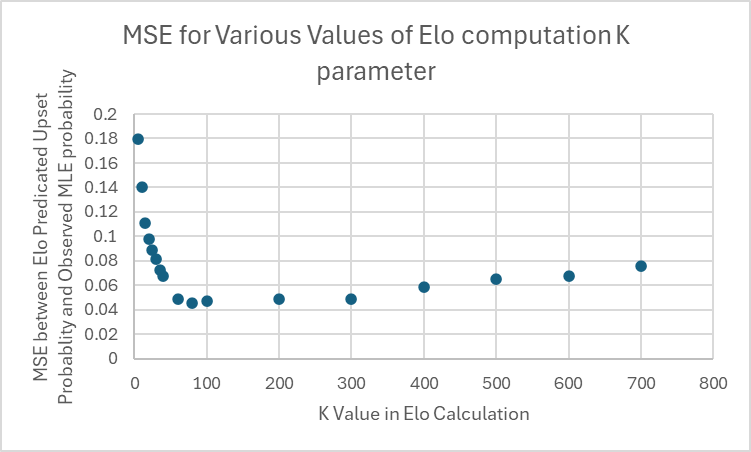
\includegraphics[width=0.5\textwidth]{MSE vs K.png}
    \end{center}
    \caption{Plot showing the effect of K on the MSE.}\label{fig:MSE vs K}
  \end{figure}

\begin{figure}[!htb]
    \begin{center}
      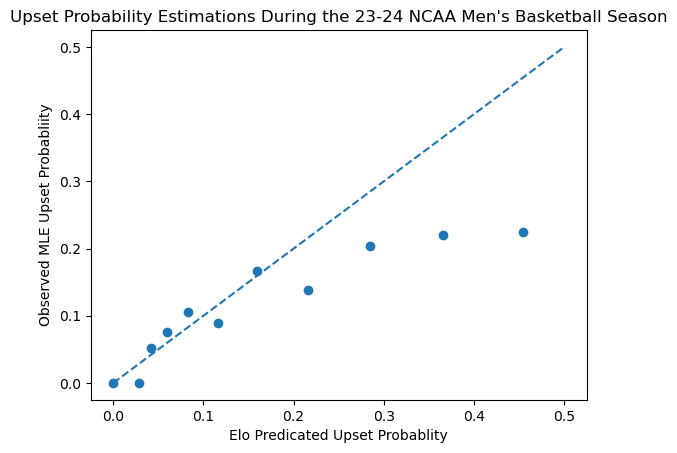
\includegraphics[width=0.5\textwidth]{Elo vs MLE.png}
    \end{center}
    \caption{Plot showing the effect of K on the MSE.}\label{fig:Elo vs MLE}
  \end{figure}

\
(Note that dots with the higher Elo upset probability estimate necessarily correspond to the partitions with smaller score differentials by definition.)

The lowest MSE was obtained when $K\approx80$ and which yielded a minimized value of $MSE\approx0.0458$. This $K$ was larger than the canonical range, which is $K \in[10, 40]$~\cite{mediumRatingSystem}. Interestingly, for this value of $K$ the Elo estimate and the MLE estimate agreed for high score differentials, but for small score differentials the Elo estimate predicted a higher probability of an upset than the MLE estimate. 

\subsection{Quantifying Uncertainty}
To first order, we now also have two (hopefully similar) ways of quantifying the measure of uncertainty in a basketball game: the expected probability of an upset based on Elo rankings (as a function of the difference in Elo rankings), and the MLE for the probability of an upset (as a function of the difference in Elo rankings). Using the expected probability as a measure of the uncertainty assumes that the formula used to calculate the expected probabilities given Elo rating is a good model for the probability of an upset. Using the bootstrapped probability as a measure of uncertainty assumes that we have enough data to be able to approximate the true probability of an upset for a given class of difference in Elo rankings. Both of these measures assume that our Elo rankings --- or at least their differences --- accurately capture the differences in skill level between teams (which is no small assumption). We will make this aassumption for the remainder of this paper; while our Elo system might not be completely accurate, it could be improved with more time and the incorporation of more data (see \autoref{nextSteps}).

As far as our ``basketball uncertainty principle'' --- that is, the uncertainty for a game between the best and the worst tournament team --- we found our bootstrapped approximate 95\% confidence interval to be between 0 and 0.05376. The fact that this includes 0 is undesirable, but perhaps could be remedied with more samples. See \autoref{fig:bootstrap dist} for the bootstrap estimated distribution of the sample mean.

Again, to interpret this as even an estimate of our actual fundamental uncertainty requires us to make significant assumptions (\autoref{bootstrapping}). There are many things we could do to increase the accuracy of this estimate, which we discuss in the final section. 

\begin{figure}[!htb]
    \begin{center}
      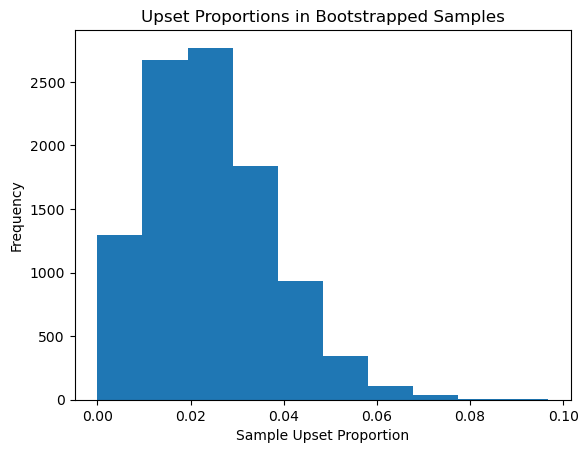
\includegraphics[width=0.5\textwidth]{Bootstrapped dist.png}
    \end{center}
    \caption{The bootstrapped distribution for the true probability of upset in the highest score differential class. 10,000 samples were drawn from the original set of games in the partition and the sample mean was calculated for each sample.}
    \label{fig:bootstrap dist}
  \end{figure}



\section{Next Steps}\label{nextSteps}
\subsection{Predicting March Madness 2024}
We would like to see how well our model could have predicted the results of the March Madness 2024 Tournament. To this end, we would have ran a large number of simulations using our Elo predictions as probabilities that each team won. We would have then recorded what percentage of times we correctly predicted the outcome of the tournament. Since this would likely be very low (if we ever got it at all) we would have also recorded the average percentage of games for which we correctly predicted the outcome. Our goal here would be to see if (on average) our model performed better than just picking the winner as the one with the better seed. Note that in the 2024 March Madness, picking the higher seed have yielded correct predictions on 41/60 of the games (not counting the preliminaries or Final Four in which there were teams with the same seed playing against each other)~\cite{wikipedia2024NCAA}.

\subsection{Overfitting}
There are several things we would have liked to check if we had had more time. For one, it would be interesting to explore the effect of overfitting by the choice of $K$. That is, does the value of $K$ which minimized the MSE for the bootstrapping verification also maximize the likelihood of predicting the actual outcome of the tournament? If not, then we may want to look into a different way of picking $K$ (perhaps one which incorporates past data) as this choice would seem to have lead to overfitting on the regular season games. Another thing we would have liked to have done is to see how our MSE estimates would change if we added noise to the data; for example, we could have multiplied each score in the game by some rangomd number between 0.8 and 1.2 and seen if we would still have obtained a similar ideal value of $K$ and the similar MSE for this value. If so, this would indicate our Elo system is robust, and that our $K$ value is not overfit to the regular season data.

\subsection{Reiterating Elo Scores}
Even without more data, we also could have likely improved the accuracy of our Elo rankings by reiterating through the season multiple times. That is, after we've reached the end of the season, we just start at the beginning and continue to update Elo rankings after each game. It would have been interesting to see if this process causes each team's Elo rankings to converge to particular values, and explore the effect of different $K$ on the relative difference between these. For example, could it be the case that despite $K$ causing the sizes of the Elo scores to change, they converge to values where the \textit{differences} between scores are approximately the same? This would indicate a robustness in the Elo system to different choices of $K$.

\subsection{Bayesian Estimation}
Second, we would have looked for a way to determine a prior distribution for the true ${p}_u(\Delta_{\text{Elo}})$ using our Elo expected ratings and then updating this prior via Bayesian inference using the observed upset game data to obtain a posterior distribution. We would have then found the maximum a posteriori (MAP) estimate (the parameter value that maximizes the posterior distribution~cite{probabilitycourseMaximumPosteriori}) for the probability of an upset in the highest score differential category.

\subsection{Confidence Intervals}
Third, we would have checked if all of the Elo expected probabilities were within approximate bootstrapped 95\% confidence intervals for $\hat{p}_u(\Delta_{\text{Elo}})$. This would have been a good sign that our Elo system is accurate. With more time, we also would have done more to explore the validity of the assumptions required for the approximate bootstrapped percentile confidence intervals to hold.

\subsection{Additional Data}\label{additionalData}
There are a few ideas we would have liked to implement if we had had more data on hand.
\begin{itemize}
    \item We would have liked to incorporate the homefield advantage in the expected score calculated from the Elo system. If we had had this data, we would have quantified the homefield advantage by finding the additional average win proportion $A$ of home teams vs that of away teams (say, over the past ten years). We would then add $A$ to the expected score of any home team in a game and subtract it from the expected score of the away team. For example, if we found that home teams on average win 53\% of games, then we would add/subtract $A=0.03$. This way, the expected score of two teams with the same Elo score would be $0.5 \pm 0.03$. 
    \item To pick the $K$ that minimizes the MSE for our Elo system compared to the observed MLE probability, we could use data from past seasons in the same way we did with the data we have now and find the $K$ that minimizes the sum of the MSEs from the different seasons. Even better, we could use the data from past tournaments, since those data may be more accurate for predicting tournament games (e.g.\ higher levels of variability due to high pressure scenario).
    \item As previously mentioned, it would have been ideal to have an accurate Elo rating for the other teams in the league, which would require regular season data for those teams.
    \item There are many ways we could improve our Elo system with individual player data. For example, one idea would be to give each of the starting members of every team an Elo score, in addition to the team itself (to quantify how well the team plays together). The expected scores would then be based on the differences in some combination of the Elo scores (perhaps a simple average of the players' scores added to the team's score). Updates would be done to the team's scores by the same method as above, while players' scores would change based on some combination of their offensive/defensive stats in the game.
\end{itemize}

\bibliographystyle{plain}
\bibliography{bibliography}

\newpage

\section{AI Use Report}
ChatGPT was used to fix bugs in our code as well as for preliminary exploration on the problem. The only ideas we used from this exploration were those which we then found true sources for and cited in the paper. Here are the prompts and responses for this exploration, along with one example from many bugfixing prompts:
\begin{enumerate}
\item OpenAI ChatGPT (Nov 16, 2024 version, ChatGPT-4) \\
Query1: how is Elo score update calculated after each game? \\
Output1: \textbf{Elo Score Update Calculation}

Elo score updates are calculated using a formula that adjusts the players' ratings based on the game outcome and the expected outcome. Here's the general process:

\textbf{1. Expected Outcome Calculation}

The expected score $E_A$ for player $A$ against player $B$ is calculated as:
\[
E_A = \frac{1}{1 + 10^{\frac{R_B - R_A}{400}}}
\]

Similarly, the expected score for player $B$ is:
\[
E_B = \frac{1}{1 + 10^{\frac{R_A - R_B}{400}}}
\]

Note that:
\[
E_A + E_B = 1
\]

\textbf{2. Game Outcome}

The actual score $S_A$ for player $A$ is:
\[
S_A =
\begin{cases}
1, & \text{if player $A$ wins,} \\
0.5, & \text{if the game is a draw,} \\
0, & \text{if player $A$ loses.}
\end{cases}
\]

The actual score for player $B$ is:
\[
S_B = 1 - S_A
\]

\textbf{3. Elo Update Formula}

The updated rating for player $A$ is calculated as:
\[
R_A' = R_A + K \cdot (S_A - E_A)
\]

Similarly, for player $B$:
\[
R_B' = R_B + K \cdot (S_B - E_B)
\]

Here:
\begin{itemize}
    \item $K$ is the K-factor, a constant that determines the weight of the update (commonly between 10 and 40, depending on the rating system),
    \item $S_A$ and $S_B$ are the actual scores,
    \item $E_A$ and $E_B$ are the expected scores.
\end{itemize}

\textbf{Example Calculation}

\textbf{Scenario:}
\begin{itemize}
    \item Player $A$: $R_A = 1600$
    \item Player $B$: $R_B = 1400$
    \item $K = 32$
    \item Player $A$ wins ($S_A = 1$, $S_B = 0$)
\end{itemize}

\textbf{Step 1: Expected Scores}
\[
E_A = \frac{1}{1 + 10^{\frac{1400 - 1600}{400}}} = \frac{1}{1 + 10^{-0.5}} \approx 0.76
\]
\[
E_B = 1 - E_A = 0.24
\]

\textbf{Step 2: Elo Updates}
\[
R_A' = 1600 + 32 \cdot (1 - 0.76) = 1600 + 7.68 \approx 1608
\]
\[
R_B' = 1400 + 32 \cdot (0 - 0.24) = 1400 - 7.68 \approx 1392
\]

\textbf{Results:}
\begin{itemize}
    \item Player $A$'s new rating: $R_A' \approx 1608$
    \item Player $B$'s new rating: $R_B' \approx 1392$
\end{itemize}

\item
Query2: where does the formula in 1 come from \\
Output2: The formula for the expected outcome in Elo rating systems has its roots in probability theory and is based on a logistic distribution. It was designed to model the likelihood of one player defeating another based on their relative skill levels.

\textbf{Key Principles Behind the Formula}

\textbf{Skill Differences Translate to Probabilities}
\begin{itemize}
    \item The Elo system assumes that each player's skill can be represented by a single number (their Elo rating).
    \item The difference in two players' ratings ($R_A - R_B$) is used to calculate the probability of one player defeating the other.
    \item Larger differences in rating indicate a higher probability of the stronger player winning, while smaller differences imply a closer match.
\end{itemize}

\textbf{Logistic Distribution}
\begin{itemize}
    \item The formula:
    \[
    E_A = \frac{1}{1 + 10^{(R_B - R_A)/400}}
    \]
    comes from using a logistic curve to map the rating difference to a probability between 0 and 1. The logistic function is a standard choice for modeling probabilities that sum to 1 because it produces a smooth, S-shaped curve.
    \item This curve reflects diminishing returns: as the rating difference increases, the stronger player’s win probability approaches but never reaches 1.
\end{itemize}

\textbf{Scaling with the 400 Constant}
\begin{itemize}
    \item The constant $400$ in the formula determines how quickly probabilities change with respect to rating differences.
    \item A 400-point difference corresponds to a win probability of approximately 90\% for the higher-rated player. This was chosen empirically based on the performance of chess players during the Elo system's development.
    \item The choice of $400$ can be adjusted for different implementations, but it remains standard in most Elo systems.
\end{itemize}

\textbf{Summing to Unity}
\begin{itemize}
    \item The expected scores $E_A$ and $E_B$ are complementary:
    \[
    E_A + E_B = 1
    \]
    \item This ensures the model is consistent with a two-player game: if one player is more likely to win, the other is equally less likely.
\end{itemize}

\textbf{Historical Development}

Arpad Elo, the creator of the Elo system, was a physicist and chess master. He designed the system based on:
\begin{itemize}
    \item Observations of chess match outcomes.
    \item The need for a probabilistic model that reflects the actual performance of players over time.
\end{itemize}

His work combined empirical data with the mathematical properties of the logistic function to create a simple yet effective rating system.

\item
Query3: why is bootstrapping useful \\
Output3: Bootstrapping is a statistical technique used to estimate the sampling distribution of a statistic by resampling with replacement from the original data. It is useful for several reasons:

\textbf{1. Doesn't Require Strong Assumptions}
\begin{itemize}
    \item Unlike traditional parametric methods, bootstrapping does not assume a specific distribution for the data (e.g., normality). This makes it applicable to a wide variety of data types and problems.
\end{itemize}

\textbf{2. Provides Robust Estimates}
\begin{itemize}
    \item It helps calculate robust estimates of standard errors, confidence intervals, and other statistical measures, even when traditional assumptions (like independence or homogeneity of variance) are violated.
\end{itemize}

\textbf{3. Useful for Small Samples}
\begin{itemize}
    \item When the sample size is small, traditional inferential techniques may not be reliable. Bootstrapping generates many simulated samples, effectively allowing a more reliable estimation.
\end{itemize}

\textbf{4. Versatile Across Statistics}
\begin{itemize}
    \item It can be applied to virtually any statistic (mean, median, variance, regression coefficients, etc.), making it a highly flexible tool.
\end{itemize}

\textbf{5. Handles Complex Data}
\begin{itemize}
    \item Bootstrapping is particularly useful for complex data structures, such as hierarchical models or situations where analytical solutions are challenging.
\end{itemize}

\textbf{6. Confidence Intervals and Hypothesis Testing}
\begin{itemize}
    \item Bootstrapping provides a straightforward way to compute confidence intervals and perform hypothesis testing without relying on asymptotic theory or approximate formulas.
\end{itemize}

\textbf{7. Improves Intuition}
\begin{itemize}
    \item By resampling the data and observing the variability of a statistic, bootstrapping provides intuitive insights into the uncertainty of estimates.
\end{itemize}

\textbf{Example}
\begin{itemize}
    \item Suppose you calculate the mean of a dataset, and you want a confidence interval for it. Instead of relying on formulas based on assumptions, you can:
    \begin{itemize}
        \item Resample the data with replacement multiple times.
        \item Compute the mean for each resample.
        \item Use the distribution of these means to derive the confidence interval.
    \end{itemize}
\end{itemize}

\textbf{Limitations}
\begin{itemize}
    \item \textbf{Computationally Intensive:} Bootstrapping involves many resampling iterations, which can be slow for large datasets or complex models.
    \item \textbf{Not Always Accurate:} In cases of very small sample sizes or heavily skewed distributions, bootstrapping may not be reliable.
    \item \textbf{Dependent on Data Quality:} If the original sample is not representative, the bootstrapped estimates may also be biased.
\end{itemize}

Despite these limitations, bootstrapping remains a powerful and widely-used tool in modern statistics.

\item
Query4: Recipe terminated with fatal error: spawn pdflatex ENOENT. \\
Output4: The error \texttt{spawn pdflatex ENOENT} typically occurs when attempting to compile a LaTeX document and the necessary LaTeX distribution (e.g., \texttt{pdflatex}) is not installed or cannot be found by the system. Here's how to resolve this issue:

\textbf{1. Check if LaTeX is Installed}
The error indicates that \texttt{pdflatex} (a part of a LaTeX distribution) is missing.

\textbf{On Windows:}
\begin{itemize}
    \item Verify that you have a LaTeX distribution installed, such as:
    \begin{itemize}
        \item MiKTeX: \url{https://miktex.org/}
        \item TeX Live: \url{https://www.tug.org/texlive/}
    \end{itemize}
    \item Ensure the LaTeX installation directory is added to your system's PATH environment variable:
    \begin{itemize}
        \item Open the "Environment Variables" settings.
        \item Locate the PATH variable and add the directory where \texttt{pdflatex.exe} is located (e.g., \texttt{C:\textbackslash Program Files\textbackslash MiKTeX\textbackslash miktex\textbackslash bin\textbackslash x64}).
    \end{itemize}
\end{itemize}

\textbf{On macOS:}
\begin{itemize}
    \item Install MacTeX: \url{https://www.tug.org/mactex/}
    \item Ensure the binary directory is in your PATH:
    \begin{itemize}
        \item Usually \texttt{/Library/TeX/texbin}.
    \end{itemize}
\end{itemize}

\textbf{On Linux:}
\begin{itemize}
    \item Install TeX Live or another distribution using your package manager:
    \begin{verbatim}
    sudo apt-get install texlive
    \end{verbatim}
    \item Check if \texttt{pdflatex} is available:
    \begin{verbatim}
    pdflatex --version
    \end{verbatim}
\end{itemize}

\textbf{2. Check Your Editor's Configuration}
If you're using an editor like VS Code or TeXstudio, ensure it's correctly configured:

\textbf{VS Code:}
\begin{itemize}
    \item Ensure you have the LaTeX Workshop extension installed.
    \item In \texttt{settings.json}, configure the LaTeX tools path, if necessary:
    \begin{verbatim}
    "latex-workshop.latex.tools": [
      {
        "name": "pdflatex",
        "command": "pdflatex",
        "args": [
          "-synctex=1",
          "-interaction=nonstopmode",
          "-file-line-error",
          "%DOC%"
        ]
      }
    ]
    \end{verbatim}
    \item Restart VS Code.
\end{itemize}

\textbf{TeXstudio:}
\begin{itemize}
    \item Go to \texttt{Options > Configure TeXstudio > Commands}.
    \item Ensure \texttt{pdflatex} is properly set, e.g., \texttt{pdflatex -synctex=1 -interaction=nonstopmode \%.tex}.
\end{itemize}

\textbf{3. Verify pdflatex Availability}
Run the following command in your terminal or command prompt:
\begin{verbatim}
pdflatex --version
\end{verbatim}
If you see the version information, it means \texttt{pdflatex} is installed and available in your PATH. If not, verify your LaTeX distribution installation or add it to the PATH.

\textbf{4. Fix Specific LaTeX Distribution Issues}
\begin{itemize}
    \item \textbf{MiKTeX:} Open the MiKTeX console and ensure all necessary packages are installed and up-to-date.
    \item \textbf{TeX Live:} Use the \texttt{tlmgr} command to update your distribution and ensure \texttt{pdflatex} is installed:
    \begin{verbatim}
    tlmgr install pdflatex
    \end{verbatim}
\end{itemize}

\textbf{5. Restart and Recompile}
\begin{itemize}
    \item After making changes:
    \begin{itemize}
        \item Restart your editor/IDE.
        \item Attempt to compile the LaTeX document again.
    \end{itemize}
\end{itemize}

If the issue persists, share more details about your setup (OS, LaTeX distribution, and editor), and I can provide further help!
    
\end{enumerate}

\end{document}




% CANT DO THIS WITHOUT KNOWING TRUE P-HAT. could do this to see how often it covers E_0 but who cares? 2. Bootstrap CI's to estiate coverage probability (what percent of the bootstrapped CI's covered the )
% Note that the probability of an upset obtained via bootstrapping $\hat{p}_u(\Delta_{\text{Elo}})$ could be anything between 0 and 1, while the expected outcome probability from Elo rankings is necessarily between 0 and 1/2. However, we expect that $\hat{p}_u(\Delta_{\text{Elo}})$ should be roughly less than 0 to 1/2, for the same reasons that we hope our Elo expected outcomes $E_u(\Delta_{\text{Elo}})$ are similar to $\hat{p}_u(\Delta_{\text{Elo}})$ for each value of $(\Delta_{\text{Elo}})$. 
